\bundlefile{lecturesight-videoanalysis-impl.jar}

The bundle provides services for real time video analysis. The implementation is responsible for finding moving objects of a certain size in the scene. In detail the bundle holds three different services

\begin{itemize}
 \item Change Detection Service
 \item Background Model and Difference Service
 \item Foreground Regions Service
\end{itemize}

The Foreground Regions Service uses the Background Model Service and the Change Detection Service to build the foreground model. The foreground model is build up over time. Regions that show minor activity are aged and removed after some time. Other services can order the Foreground Service to exclude regions from this mechanism. Also other services can order the Foreground Service to immediately discard a foreground region.

\image{img-videoanalysis}{The video analysis process}{
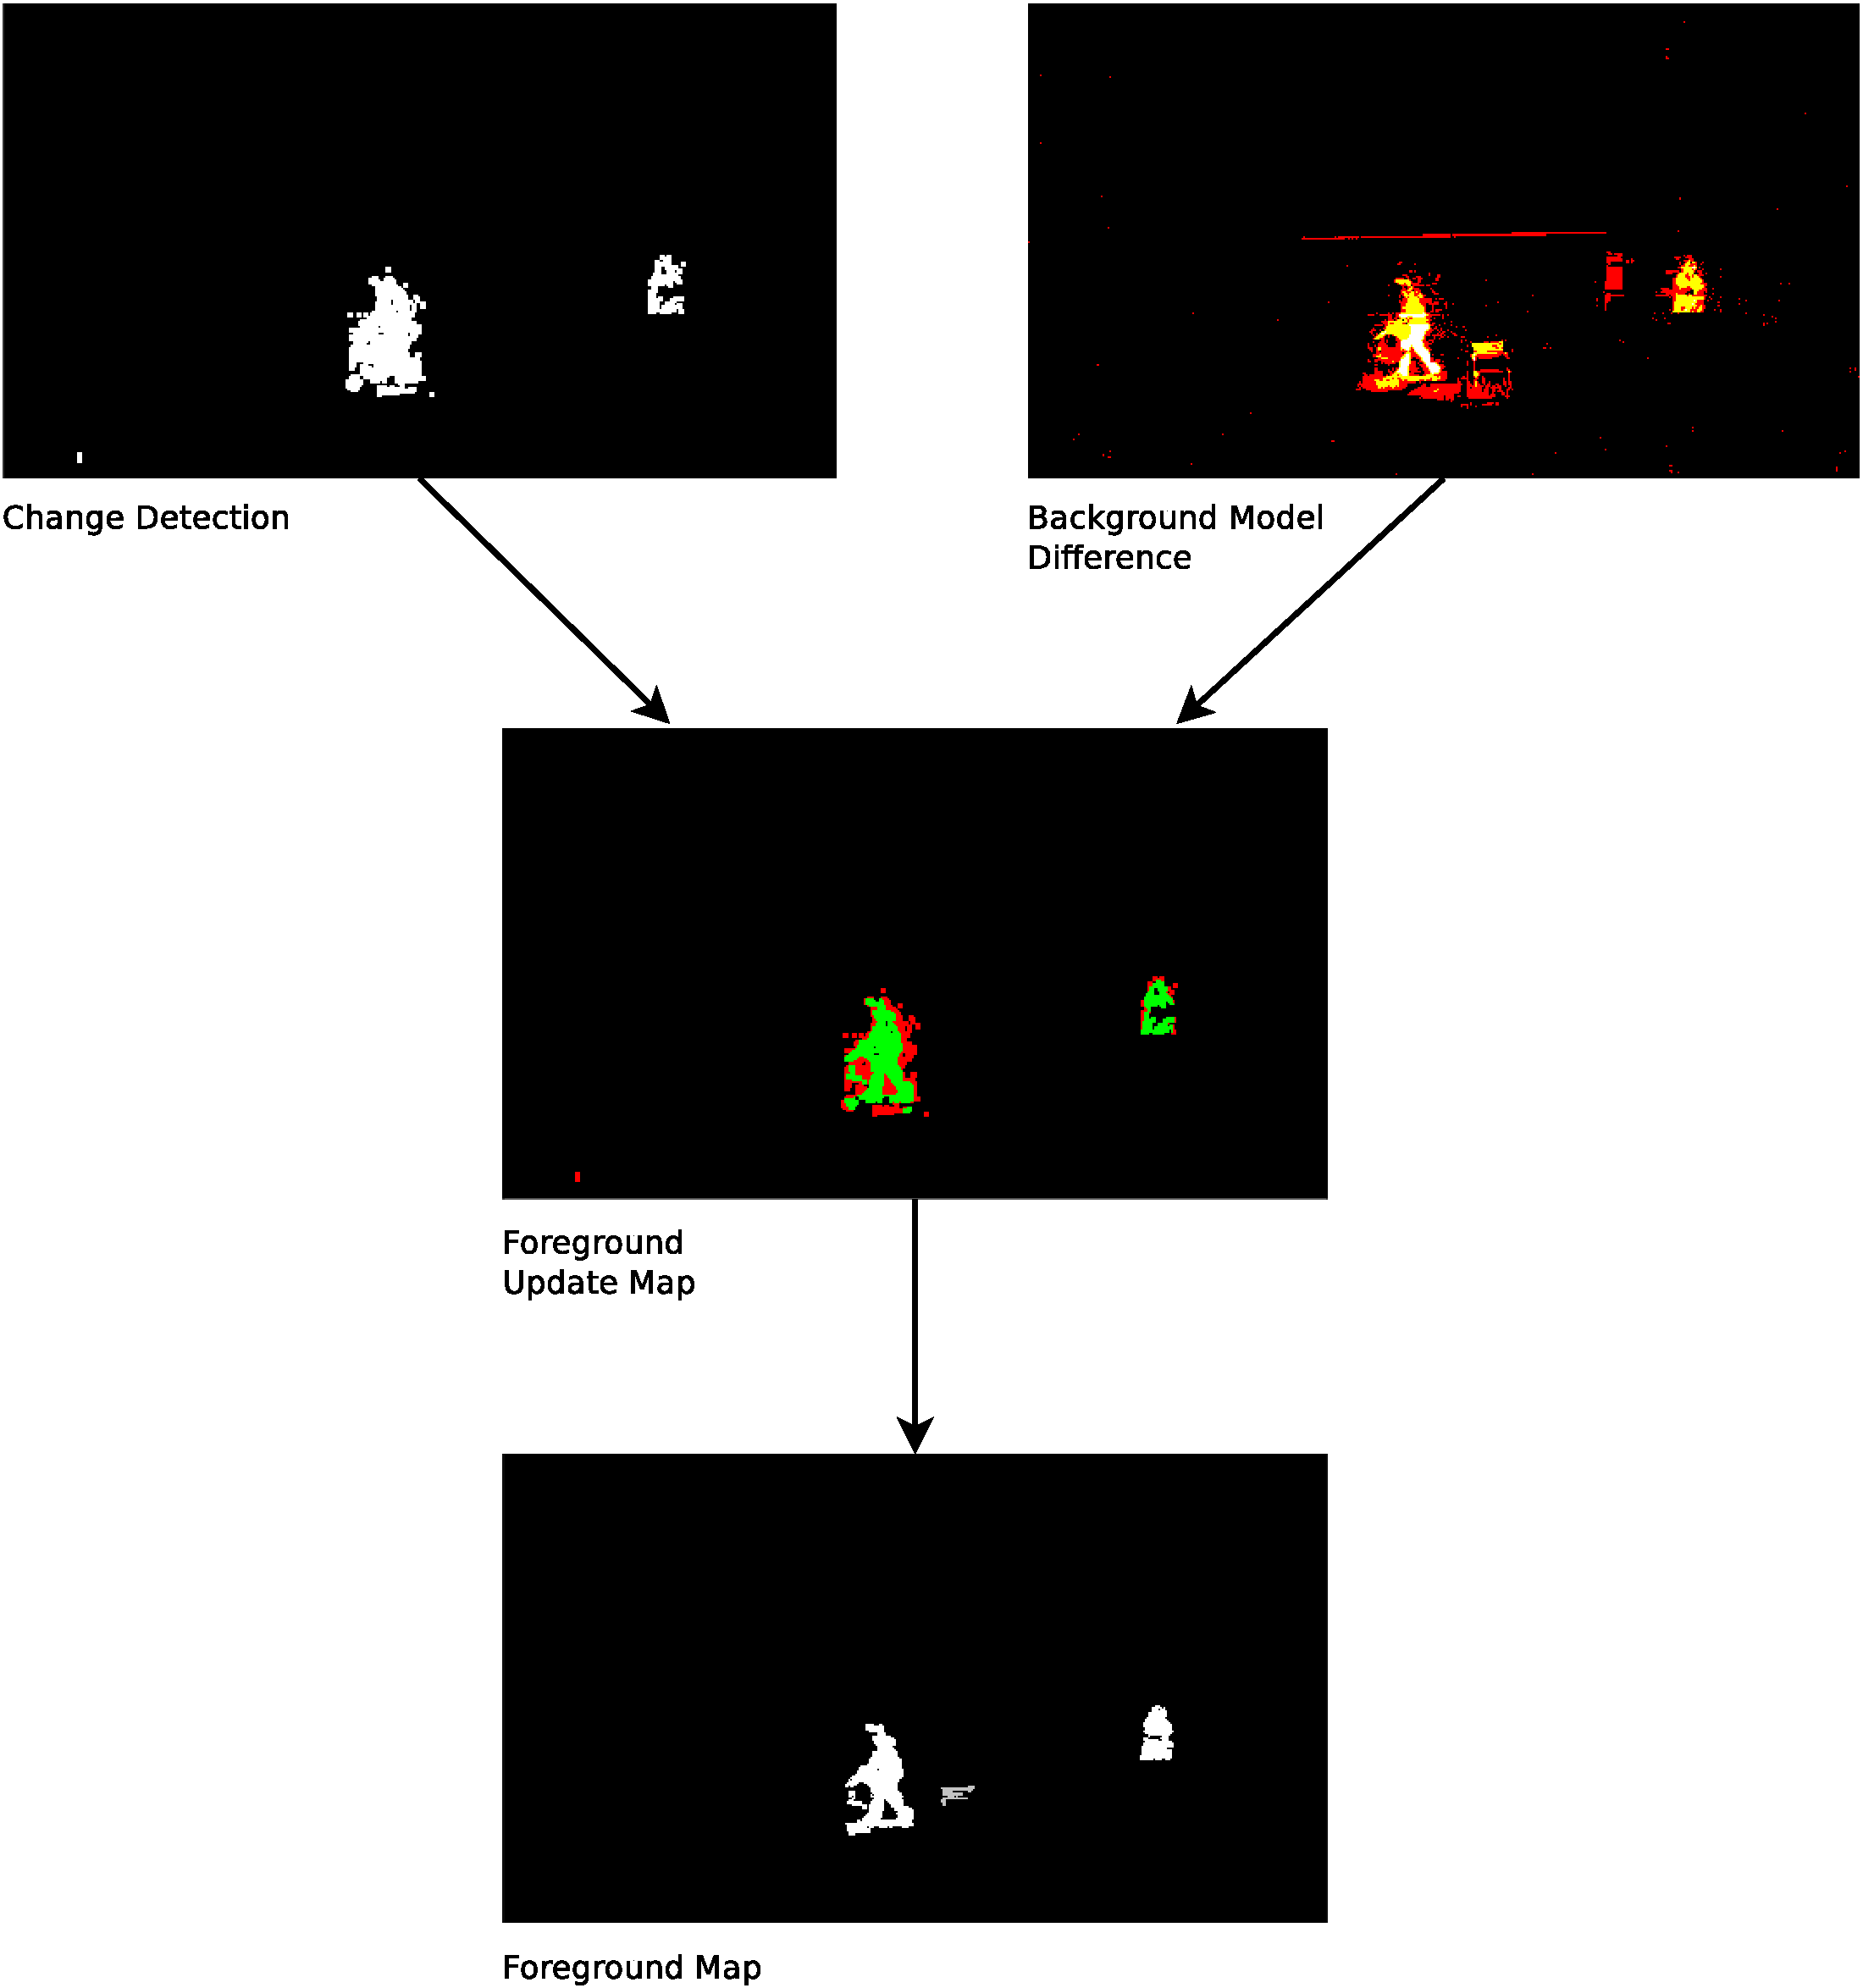
\includegraphics[width=0.9\textwidth]{../modules/lecturesight-videoanalysis-impl/manual/videoanalysis.pdf}
}

\subsubsection{Console Commands}

\consolecommand{fg:reset}{no arguments}{Re-initializes the Foreground Model.}

\consolecommand{bg:reset}{no arguments}{Re-initializes the Background Model.}

\configproperties

\property{cv.lecturesight.videoanalysis.changedetect.threshold}{18}{
$[0 \dots 255]$ Threshold for the change detection. Lower values yield detection of slighter chnages in the scene.
}

\property{cv.lecturesight.videoanalysis.background.threshold.low}{30}{
$[0 \dots 255]$ Low threshold for background differencing.}

\property{cv.lecturesight.videoanalysis.background.threshold.mid}{120}{
$[0 \dots 255]$ Mid threshold for background differencing.}

\property{cv.lecturesight.videoanalysis.background.threshold.high}{220}{
$[0 \dots 255]$ High threshold for background differencing.}

\property{cv.lecturesight.videoanalysis.background.update.alpha}{0.5}{
$[0.0 \dots 1.0]$ Factor for the background model update. The higher the value, the faster is the update of the background model. A value of 0.0 yields no update at all. A value 1.0 yields a background model that basically is always equal to the preceding frame.}

\property{cv.lecturesight.videoanalysis.foreground.ccl.maxblobs}{1000}{
$[1 \dots \text{MAX\_INT}]$ Maximum number of connected components that the Connected Component Analysis can discover. This value exists merely due to technical reasons.}

\property{cv.lecturesight.videoanalysis.foreground.ccl.blobsize.min}{20}{
$[1 \dots \text{MAX\_INT}]$ Minimum number of pixels a region in the foreground map must consist of to be taken up for further analysis in the Foreground Service. Regions smaller than this are discarded very early in the analysis process.
\\~\\
\noindent\textbf{Note: This value is useful for filtering out small artifcats that result from noise in the camera sensor. Also this value should be adjusted when working with video streams of high resolution because with the image size also the size of artifacts rises.} 
}

\property{cv.lecturesight.videoanalysis.foreground.ccl.blobsize.max}{10000}{
$[1 \dots \text{MAX\_INT}]$ Maximum number of pixels a region in the foreground map can consist of to be taken up for further analysis in the Foreground Service. Changes in the scene that have an unplausible size are filtered out by this value.}

\property{cv.lecturesight.videoanalysis.foreground.decay.threshold}{0.04}{
$[0.0 \dots 1.0]$ Minimum pixel activity ration ($N_{\text{chnaged}} / N$) for a region to be protected from aging in the current iteration.}

\property{cv.lecturesight.videoanalysis.foreground.decay.alpha}{5}{
$[1 \dots \text{MAX\_INT}]$ The value by which the intensity of a region is decreased when aging. Note that intensity values in the foreground map are in $[0 .. 255]$.}

\property{cv.lecturesight.videoanalysis.foreground.decay.phantom.thresh}{5}{
$[0 \dots 255]$ Threshold for phantom removal. If a pixel at the edge of a region has a neighbour that is less similar than this threshold, the pixel is removed from the foreground map. 

This mechanism helps in situation where, for example, a static object like a chair, that was part of the background model is moved. The resulting fals positive detections often show greater regions that are similar or equal to the sorrounding background (in contrast to correct detections).}
